\documentclass[accentcolor=tud7b,noresetcounter]{tudbeamer}

\usepackage[ngerman]{babel}
\usepackage[utf8]{inputenc}
\usepackage[T1]{fontenc}

% footmisc behebt u.a. Probleme mit Fu?noten in Abschnittstiteln
\usepackage[stable]{footmisc}

% Einbinden von Grafiken erm?glichen
\usepackage{graphicx}

% Paket xtab erm?glicht Umbrechen von langen Tabellen
\usepackage{xtab}
\usepackage{tikz}

% picins erlaubt das Umflie?en von Abbildungen durch Text
% Untenstehendes renewcommand behebt den picins-bug, dass Abbildungen
% nicht im Abbildungsverzeichnis auftauchen
%\usepackage{picins}
\makeatletter
%\renewcommand\piccaption{\@dblarg{\@piccaption}}
\makeatother

\usepackage{verbatim}

% Paket setspace erlaubt Umschalten auf 1.5fachen Zeilenabstand
\usepackage{setspace}

\usepackage{hyperref}
\usepackage{listings}
\usepackage{amssymb}
\usepackage{newclude}
\usepackage{multirow}
\usepackage{array}
\usepackage{tabularx}
\usepackage{hyperref} 
\usepackage{graphicx}
\usepackage{pgfplots}
\usepackage{csvsimple}
%Erm?glicht Hyperlinks zwischen Textstellen und zu externen Dokumenten
%% breaklinks=true/false: Gibt an, ob Links umgebrochen werden d?rfen.
%% linktocpage=true/false: im Inhaltsverzeichnis sind nur die Seitenzahlen
%% links, nicht der Text
%% colorlinks=true/false: Links werden eingef?rbt (Farben werden mit
%% linkcolor, anchorcolor \dots festgelegt)
%% linkcolor=Farbe: Farbe des verlinkten Textes, Dokument-interne Links
%% citecolor=Farbe: Farbe des verlinkten Textes, Links zum
%% Literaturverzeichnis
%% filecolor=Farbe: Farbe des verlinkten Textes, Links auf lokale Dateien
%% urlcolor=Farbe: Farbe des verlinkten Textes, externe URLs
%% frenchlinks=true/false: Links werden als smallcaps, anstatt farbig
%% dargestellt.
%% breaklinks=true/false: Gibt an, ob Links umgebrochen werden d?rfen.
\hypersetup{%
  linktocpage=true,
  breaklinks=true,
  colorlinks=true,
  citecolor=black,
  urlcolor=black,
  linkcolor=black,
  pdfpagemode=UseThumbs,
  pdftitle=Übung 2 - Webmining,
  pdfauthor=Ingo Adrian und Steffen Pegenau,
  pdfsubject=Webmining,
  %pdfkeywords=xy
}


\lstset{ %
  %backgroundcolor=\color{white},   % choose the background color; you must add 
%\usepackage{color} or \usepackage{xcolor}
  %basicstyle=\footnotesize,        % the size of the fonts that are used for 
					%the code
  %breakatwhitespace=false,         % sets if automatic breaks should only 
%happen at whitespace
  breaklines=true,                 % sets automatic line breaking
  %captionpos=b,                    % sets the caption-position to bottom
  commentstyle=\bf,    % comment style
  %deletekeywords={...},            % if you want to delete keywords from the 
%given language
  %escapeinside={\%*}{*)},          % if you want to add LaTeX within your code
  %extendedchars=true,              % lets you use non-ASCII characters; for 
%8-bits encodings only, does not work with UTF-8
  frame=single,                    % adds a frame around the code
  %keepspaces=true,                 % keeps spaces in text, useful for keeping 
%indentation of code (possibly needs columns=flexible)
  %keywordstyle=\color{blue},       % keyword style
  language=html,                 % the language of the code
  %otherkeywords={*,...},            % if you want to add more keywords to the 
%set
  numbers=left,                    % where to put the line-numbers; possible 
%values are (none, left, right)
  %numbersep=5pt,                   % how far the line-numbers are from the code
  %numberstyle=\tiny\color{mygray}, % the style that is used for the 
%line-numbers
  %rulecolor=\color{black},         % if not set, the frame-color may be changed 
%on line-breaks within not-black text (e.g. comments (green here))
  %showspaces=false,                % show spaces everywhere adding particular 
%underscores; it overrides 'showstringspaces'
  %showstringspaces=false,          % underline spaces within strings only
  %showtabs=false,                  % show tabs within strings adding particular 
%underscores
  %stepnumber=2,                    % the step between two line-numbers. If it's 
%1, each line will be numbered
  %stringstyle=\color{mymauve},     % string literal style
  tabsize=4,                       % sets default tabsize to 2 spaces
  %title=\lstname                   % show the filename of files included with 
%\lstinputlisting; also try caption instead of title
}

% bibtex
%\usepackage[backend=biblatex]{biblatex}

%\bibliography{refs}
%\addbibresource{refs.bib}

%%%%%%%%%%%%%%%%%%%%%%%%%%%%%%%%%%%%%%%%%%%%%%%%%%%%%%%%%%%%%%%%%%%%%%%%%%%%%%%%%%%%%%

\title%[Klima \& Geographie] % (optional, only for long titles)
{Web Mining: Übung 2}
\subtitle{Lösungsvorschlag}

\author[Ingo Adrian und Steffen Pegenau]{}
\institute[Fachbereich Informatik]{}
\date[\today]
%%%%%%%%%%%%%%%%%%%%%%%%%%%%%%%%%%%%%%%%%%%%%%%%%%%%%%%%%%%%%%%%%%%%%%%%%%%%%%%%%%%%%

\pgfplotsset{compat=1.12}

\begin{document}




  
  \begin{titleframe}
  \end{titleframe}
  
  \begin{frame}
	\frametitle{Inhaltsverzeichnis}
	\tableofcontents
  \end{frame}
  
  \begin{frame}
	\frametitle{Aufgabe 1: Spracherkennung\\
	Theorie}
	\begin{itemize}
		\item Zwei Listen: Liste mit ermittelten Buchstaben/-paaren und Referenzliste(n)
		\item Vergleiche Position der Buchstaben(-paare) mit denen der Referenzlisten
		\item Ermittlung eines Scores für jede Referenzsprache:
			\begin{itemize}
				\item Ermittle Differenz d der beiden Positionen
				\item addiere $$\frac{1}{1 + d}$$ zum Score
				\item Höchster Score hat die größte (?) Übereinstimmung von Buchstaben/-paaren
			\end{itemize}
	\end{itemize}
  \end{frame}  
  
  \begin{frame}
	\frametitle{Aufgabe 1: Spracherkennung\\
	Praxis}
	\texttt{1 german\\
	2 english\\
	3 english\\
	4 spanish\\
	5 german\\
	6 spanish\\
	7 spanish\\
	8 english\\
	9 german\\
	10 german\\}
	\vspace{\fill}
	Referenzlisten für Monogramme: {\small https://de.wikipedia.org/wiki/Buchstabenhäufigkeit}\\
	Referenzlisten für Bigramme: {\small http://practicalcryptography.com/cryptanalysis/letter-frequencies-various-languages/}
	
  \end{frame}
  \begin{frame}[t]
  	\frametitle{Aufgabe 2: Entwicklung eines Crawlers\\
  	%\hline \\
	Histogramm: Es gibt $y$ Seiten mit $x$ Links}
	%\begin{figure}[ht]
	%\begin{center}
	\resizebox {\columnwidth} {180pt} {
	\begin{tikzpicture}
	\begin{axis}[
		%xmin=0,xmax=700
	]
	\addplot table 
	[x=countOfLinks, y=countOfPages,col sep=semicolon, only marks]
	%,col sep=semicolon
	{../aufg02/linksPerPage.csv};
	\end{axis}
	\end{tikzpicture}}
	%\caption{Die Anzahl von Seiten ($y$-Achse) mit einer Anzahl Links 
	%($x$-Achse}
	%\label{fig:linksPerPage}
	%\end{center}
	%\end{figure}
  \end{frame}
  
  \begin{frame}[t]
  	\frametitle{Aufgabe 2: Entwicklung eines Crawlers\\
  	%\hline \\
	Histogramm: Es gibt x Links, die y mal auftraten}
	%\begin{figure}[ht]
	%\begin{center}
	\resizebox {\columnwidth} {180pt} {
	\begin{tikzpicture}
	\begin{axis}[
		%xmin=0,xmax=700
	]
	\addplot table 
	%timesOfLinkReference;countOfTheseLinks
	[x=timesOfLinkReference, y=countOfTheseLinks,col sep=semicolon, only marks]
	%,col sep=semicolon
	{../aufg02/unfilteredLinks.csv};
	\end{axis}
	\end{tikzpicture}}
	%\caption{Die Anzahl von Seiten ($y$-Achse) mit einer Anzahl Links 
	%($x$-Achse}
	%\label{fig:linksPerPage}
	%\end{center}
	%\end{figure}
  \end{frame}
  
\begin{frame}[t,fragile]
  	\frametitle{Aufgabe 2: Entwicklung eines Crawlers\\Erkennung wiederkehrender Links}
	\begin{itemize}
	 \item Entfernung aller Listen:
\begin{lstlisting}
<ul>
  <li><a href="start.html">Start</a></li>
  <li><a href="news.html">News</a></li>
  <li><a href="impressum.html">Impressum</a></li>
</ul>
\end{lstlisting}
\item Entfernung mit CSS-Selektor: \texttt{[class*='nav']}:
\begin{lstlisting}
<div class="main-navigation">
  ...
</div>
\end{lstlisting}
\item Speichern der HTML-Dateien als \texttt{HASH(Kanonisierte URL).html}
\end{itemize}
\end{frame}

     
 \begin{frame}[t]
  	\frametitle{Aufgabe 2: Entwicklung eines Crawlers\\
  	Wirksamkeit der Duplikaterkennung\\Es gibt x Links, die y mal auftraten}

 
	%\begin{comment}
	\resizebox {\columnwidth} {180pt} {
	\begin{tikzpicture}
	\begin{axis}[samples=20,
	xmin=-1,
	xmax=30,
  %xlabel={Links zu einem Ziel, die x mal plaziert waren...},
  %ylabel={...gab es y-Mal},
  xlabel style={below},
  ylabel style={above left},
  axis x line=center,
  axis y line=center,]%[xmin=-0.5,xmax=9,samples=10,restrict y to domain =-20:100]%
	\addplot table [x=timesOfLinkReference, y=countOfTheseLinks,col sep=semicolon, only marks] {../aufg02/unfilteredLinks.csv};
	\addplot table [x=timesOfLinkReference, y=countOfTheseLinks,col sep=semicolon, only marks] {../aufg02/filteredLinks.csv};
	\end{axis}
	\end{tikzpicture}
	}
	%\end{comment}
\end{frame}
	

  \begin{frame}[t]
  	\frametitle{Aufgabe 2: Entwicklung eines Crawlers\\
  	Wie oft wurden Hosts besucht?\\
  	(Subdomains subsumiert, Seiten: 1.107)}
  	
  	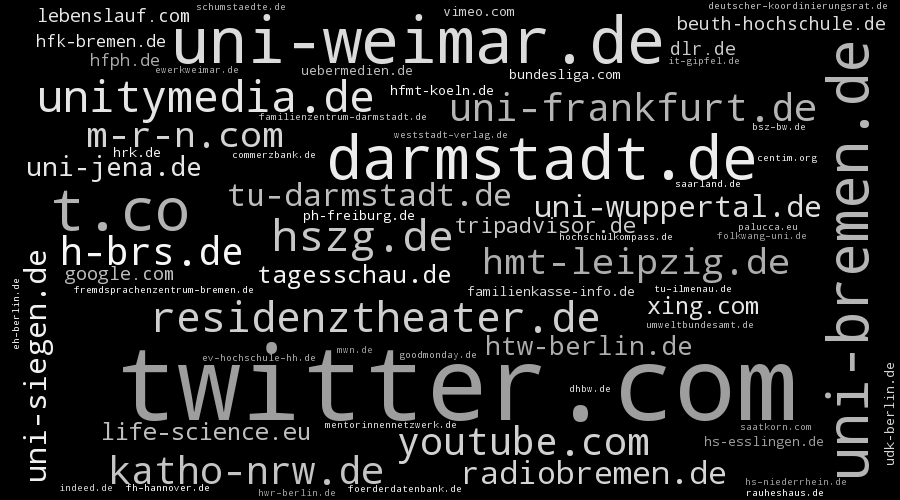
\includegraphics[width=\columnwidth, height=180pt]{../aufg02/wordcloud}	
  \end{frame}

  \begin{frame}
  	\frametitle{Verteilung gefundener Sprachen}
  	tbd
  \end{frame}
  
  \begin{frame}
  	\frametitle{Aufgabe 2: Entwicklung eines Crawlers\\Erfahrungen \& Probleme}
  	\begin{itemize}
		\item Suchstrategie funktioniert; die besuchten Hosts streuen
		\item Darstellung der Verlinkungen zwischen den Hosts wäre spannend ("`Wie vernetzt sind Hochschulen?"')
		\item Extrem häufig verlinkte Social Media Seiten erschweren solche Analysen. Bsp.: Anteil Twitter in offenen Links zu einem fortgeschrittenen Zeitpunkt: 
			$$\frac{8736}{24877}  \approx  35\%$$
  		\item Technische Lösung skaliert erwartungsgemäß nicht. Datenverwaltung nimmt mehr Zeit in Anspruch als Download:
			\begin{itemize}
				\item Zu besuchende Links und Statistiken in Textdateien
				\item Speichern eines jeden Datums direkt nach Erhebung (Persistenz)
			\end{itemize}

  	\end{itemize}

  \end{frame}
  
  \begin{frame}
  	\frametitle{Aufgabe 4: Größe des Webs \\Idee}
  	\begin{enumerate}

  	 \item Abschätzung des Index über Suchbegriff "`a"' als häufigstes Wort im Englischen in beiden Suchmaschinen
  	 \item Suche nach "`Darmstadt ESOC"' (relativ wenige Ergebnisse)
  	 \item Crawlen des Suchergebnisses um die gemeinsame Menge zu bestimmen
  	 \item Ergebnisse:\\
  	 \begin{tabular}{|l|r|r|c|}
	  \hline
	  \textbf{Name ($i$)} & \textbf{$s_i$ ("`Index"')} & \textbf{$n_i$ (Ergebnisse)} & \textbf{$n_0$ (gem. Ergebnisse)}\\
	  \hline
	  Google ($g$) & 25.270.000.000 & 117.000 & \multirow{ 2}{*}{\Huge{?}}\\
	  Bing ($b$)  & 140.000.000 & 72.800 & \\
	  \hline
  	\end{tabular}
  	\item Größe des Webs:
  	$$N \approx s_g \frac{n_b}{n_0} \approx s_b \frac{n_g}{n_0}$$
  	\end{enumerate}
  \end{frame}
  \newenvironment{allintypewriter}{\ttfamily}{\par}
  \begin{frame}
      \frametitle{Aufgabe 4: Größe des Webs \\Problem: Googles Heuchelei oder\\ Crawlen ohne gecrawled zu werden}
      \begin{itemize}
       \item 
       \begin{allintypewriter}
       "`About this page

	Our systems have detected unusual traffic from your computer network. This page checks to see if it's really you sending the requests, and not a robot. Why did this happen?"'
       \end{allintypewriter}
	$$\Rightarrow n_0 \text{ schätzen}$$ 
	\begin{tabular}{|l|r|r|c|}
	  \hline
	  \textbf{Name ($i$)} & \textbf{$s_i$ ("`Index"')} & \textbf{$n_i$ (Ergebnisse)} & \textbf{$n_0$ (gem. Ergebnisse)}\\
	  \hline
	  Google ($g$) & 25.270.000.000 & 117.000 & \multirow{ 2}{*}{\large{$1 \leq n_0 \leq 72.800$}}\\
	  Bing ($b$)  & 140.000.000 & 72.800 & \\
	  \hline
  	\end{tabular} \\
  	\hfill \\
  	\hfill \\
  	\begin{tabular}{rrrcll}
  	 & & Minimal & & Maximal & \\
  	 $N\approx s_g \frac{n_b}{n_0} = $ & $[$ & $0,000253 \cdot 10^{15}$ & ; & $1,84 \cdot 10^{15}$ & $]$ \\
  	 $N\approx s_b \frac{n_g}{n_0} = $ & $[$ & $0,00000225 \cdot 10^{15}$ & ; & $0,0164 \cdot 10^{15}$ & $]$ 
  	\end{tabular}
      \end{itemize}
  \end{frame}
  
  \begin{frame}
    \frametitle{Aufgabe 4: Größe des Webs \\Lösung \& Interpretation}
    \begin{tabular}{rrrcll}
  	 & & Minimal & & Maximal & \\
  	 $N\approx s_g \frac{n_b}{n_0} = $ & $[$ & $0,000253 \cdot 10^{15}$ & ; & $1,84 \cdot 10^{15}$ & $]$ \\
  	 $N\approx s_b \frac{n_g}{n_0} = $ & $[$ & $0,00000225 \cdot 10^{15}$ & ; & $0,0164 \cdot 10^{15}$ & $]$ 
    \end{tabular} \\
  	\hfill \\
  	\hfill \\
    In Worten: \\
    \begin{tabular}{rrrcll}
  	 & & Minimal & & Maximal & \\
  	 $N\approx s_g \frac{n_b}{n_0} = $ & $[$ & 25 Milliarden & ; & 1,84 Billiarden & $]$ \\
  	 $N\approx s_b \frac{n_g}{n_0} = $ & $[$ & 225 Millionen & ; & 16 Billionen & $]$ 
    \end{tabular} \\
    \hfill \\
    Laut \url{http://www.worldwidewebsize.com/} sind es etwa 50 Milliarden Seiten. Diese Zahl liegt im Rahmen dieser Schätzung. Aber Präzision sieht anders aus.
 \end{frame}


  
  
  %\begin{frame}
   % \frametitle{Quellen}
    
    %\printbibliography
  %\end{frame}

% etc
\end{document}